\chapter{Case-studie: Avstandsoppfølging i Trondheim kommune}
\label{ch:case}

\section{Bakgrunn}
\blindtext

\section{Eksisterende løsning}
\blindtext

\begin{figure}
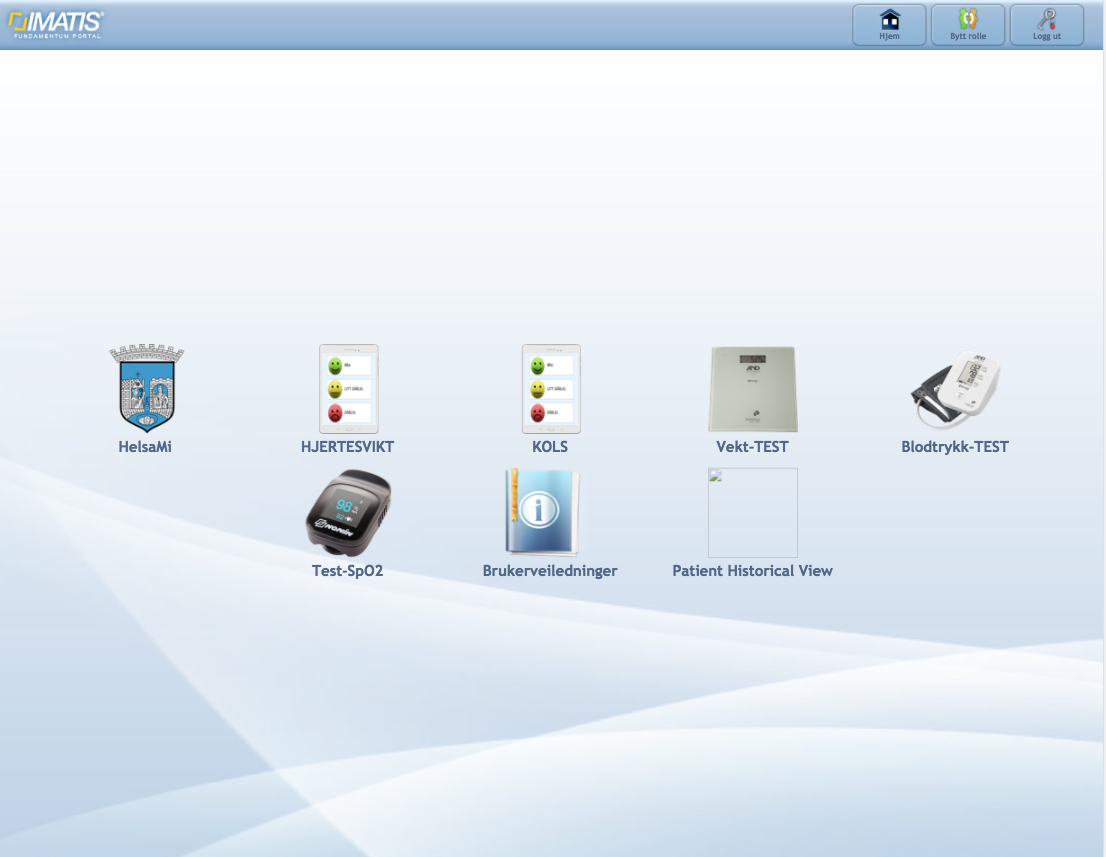
\includegraphics[width=1.0\textwidth,center]{fig/helsami/tk_1_start}
\caption{asdfasd sad}
\label{fig:helsami1}
\end{figure}

\begin{figure}
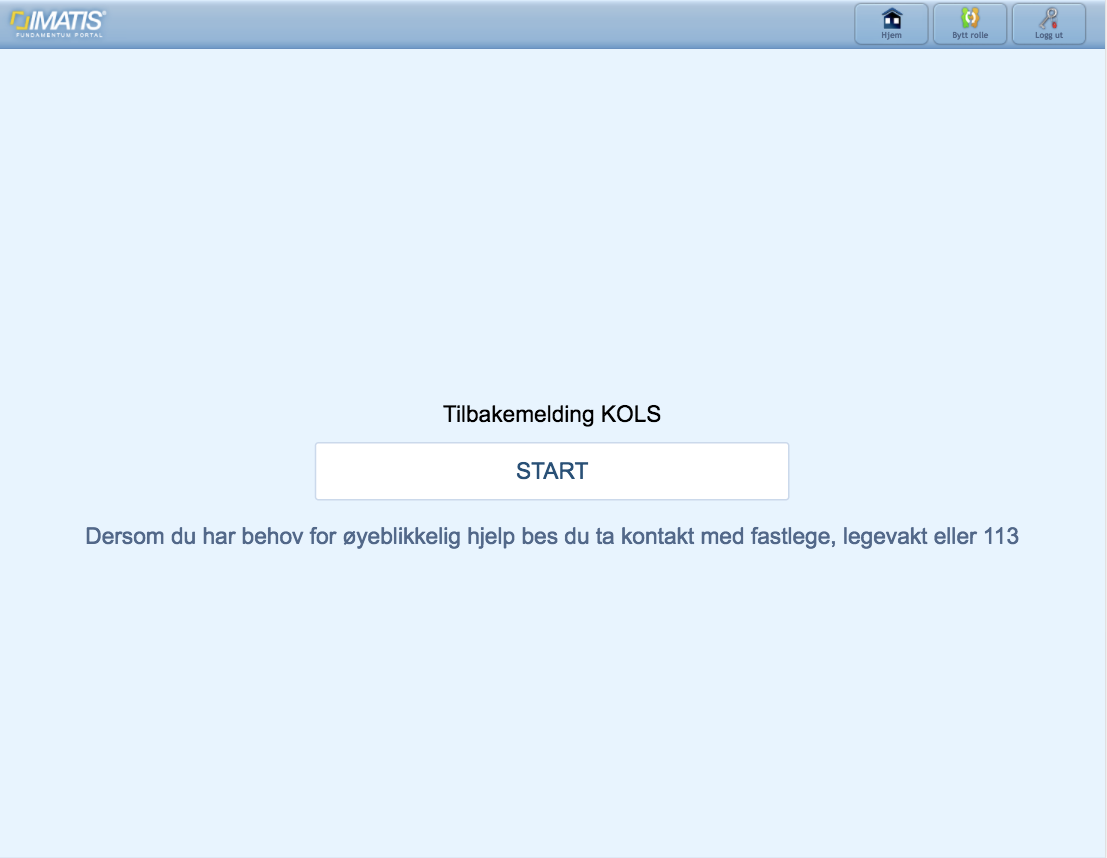
\includegraphics[width=1.0\textwidth,center]{fig/helsami/tk_2_kols}
\caption{asdfasd sad}
\label{fig:helsami1}
\end{figure}

\begin{figure}
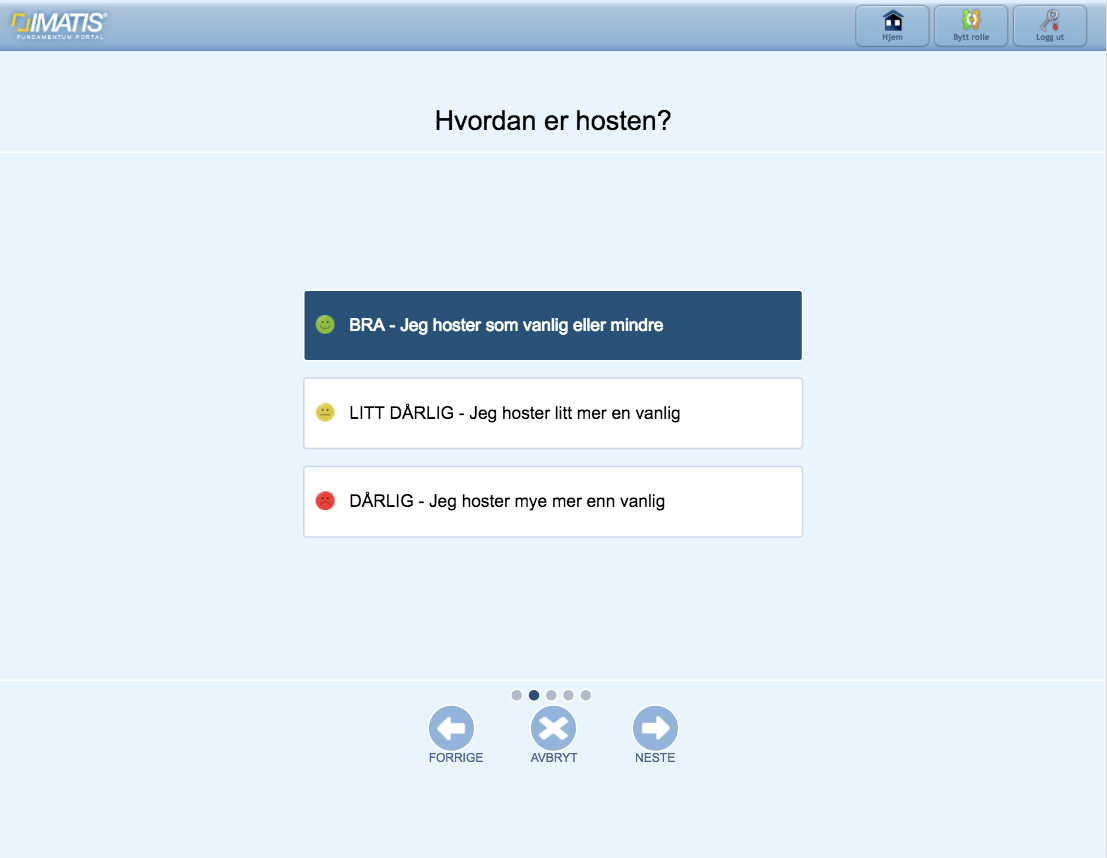
\includegraphics[width=1.0\textwidth,center]{fig/helsami/tk_3_kols}
\caption{asdfasd sad}
\label{fig:helsami1}
\end{figure}

\begin{figure}
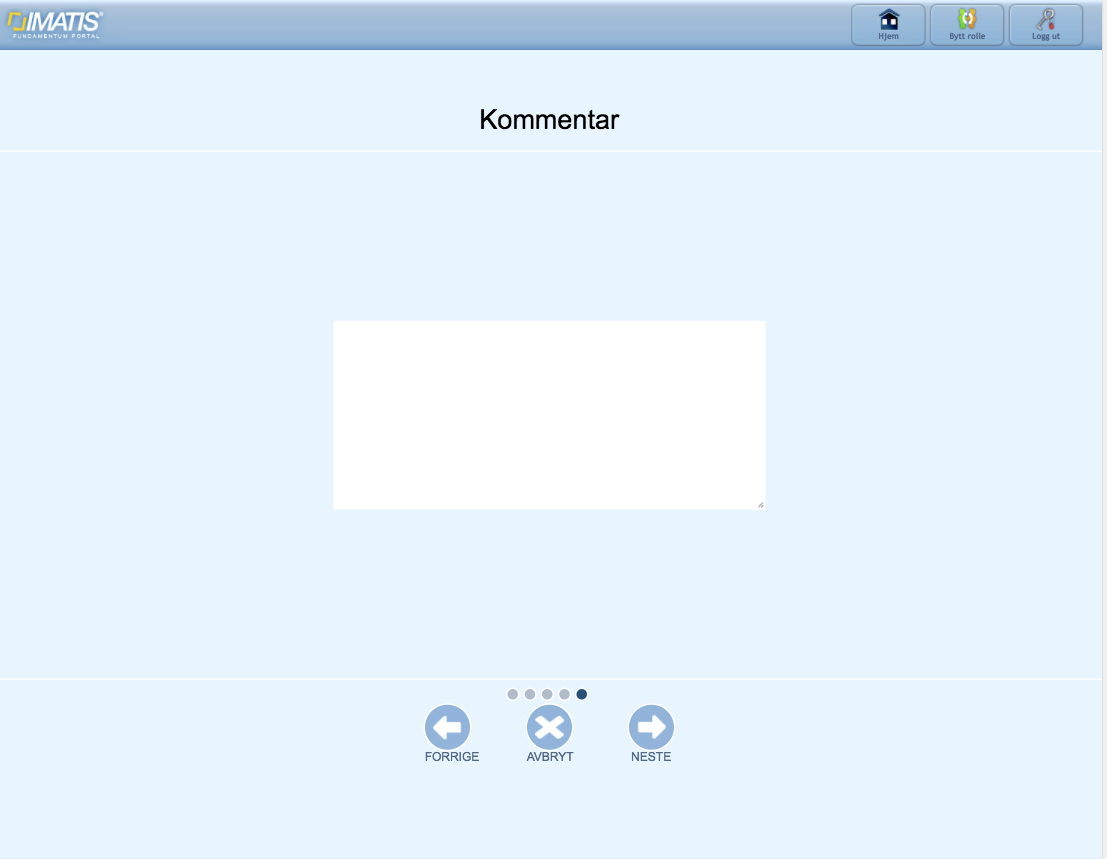
\includegraphics[width=1.0\textwidth,center]{fig/helsami/tk_6_kols}
\caption{asdfasd sad}
\label{fig:helsami1}
\end{figure}

\begin{figure}
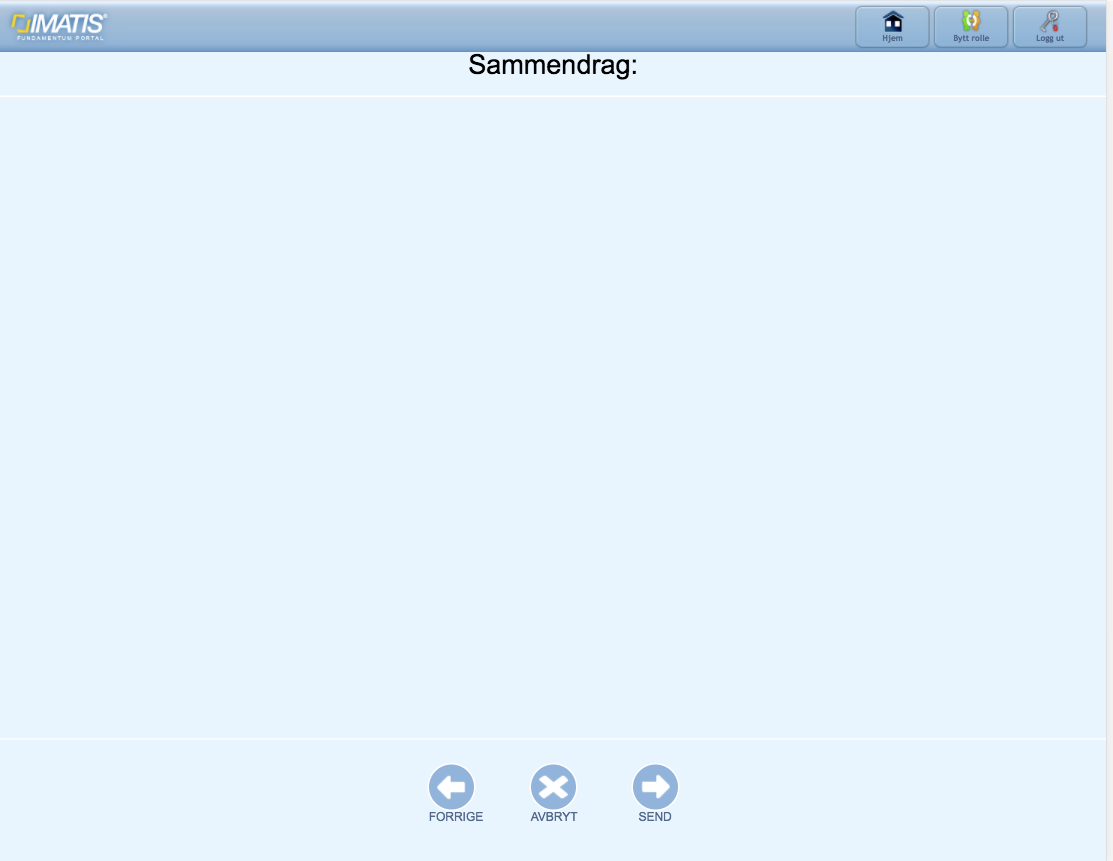
\includegraphics[width=1.0\textwidth,center]{fig/helsami/tk_7_kols}
\caption{asdfasd sad}
\label{fig:helsami1}
\end{figure}

\begin{figure}
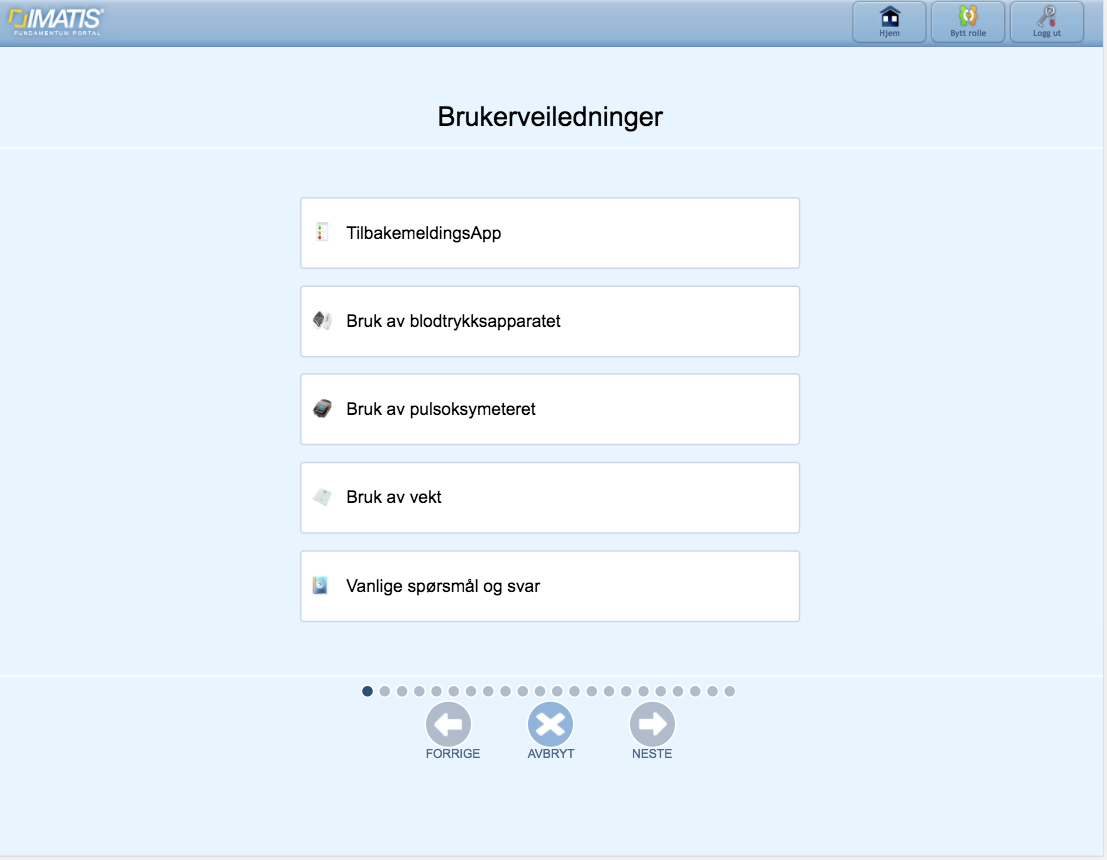
\includegraphics[width=1.0\textwidth,center]{fig/helsami/tk_8_brukerveil}
\caption{asdfasd sad}
\label{fig:helsami1}
\end{figure}

\begin{figure}
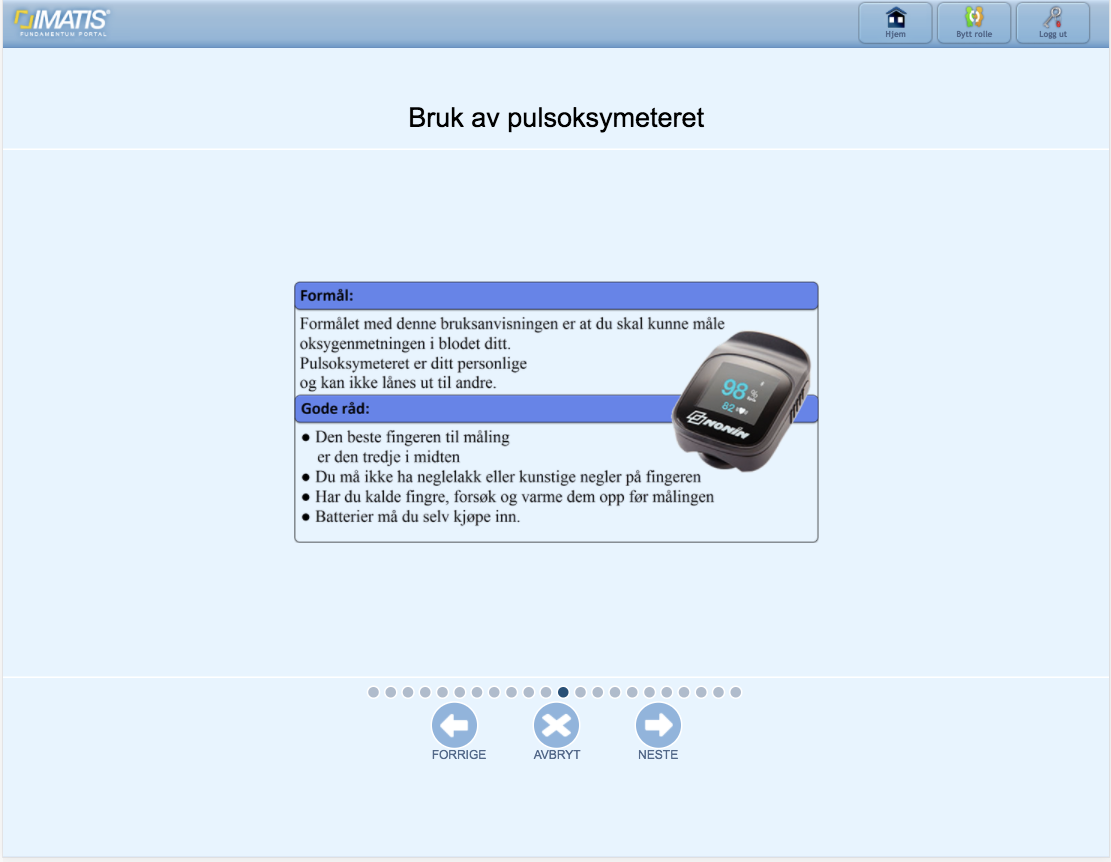
\includegraphics[width=1.0\textwidth,center]{fig/helsami/tk_9_brukerveil_puls}
\caption{asdfasd sad}
\label{fig:helsami1}
\end{figure}

\begin{figure}
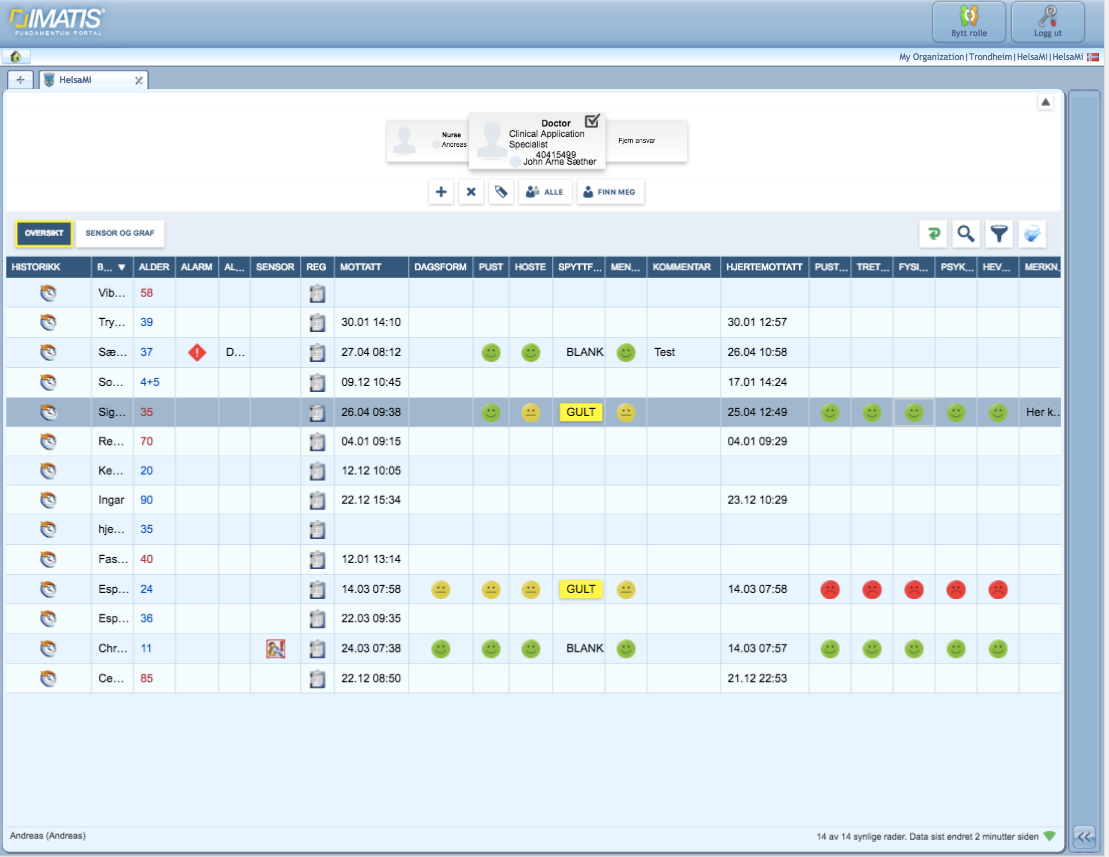
\includegraphics[width=1.0\textwidth,center]{fig/helsami/tk_10_oversikt}
\caption{asdfasd sad}
\label{fig:helsami1}
\end{figure}

\begin{figure}
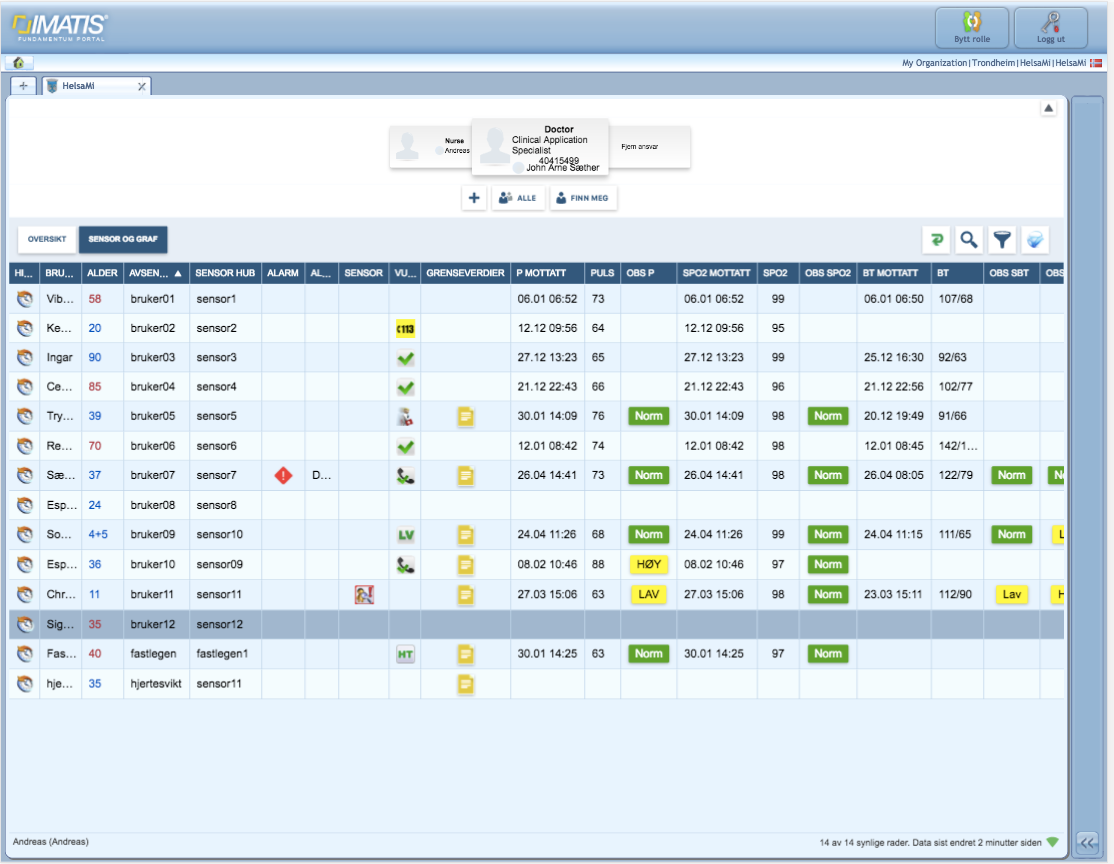
\includegraphics[width=1.0\textwidth,center]{fig/helsami/tk_11_sensoroggraf}
\caption{asdfasd sad}
\label{fig:helsami1}
\end{figure}

\section{Fremtidige planer}
